
\begin{figure*}[t!]
\centering
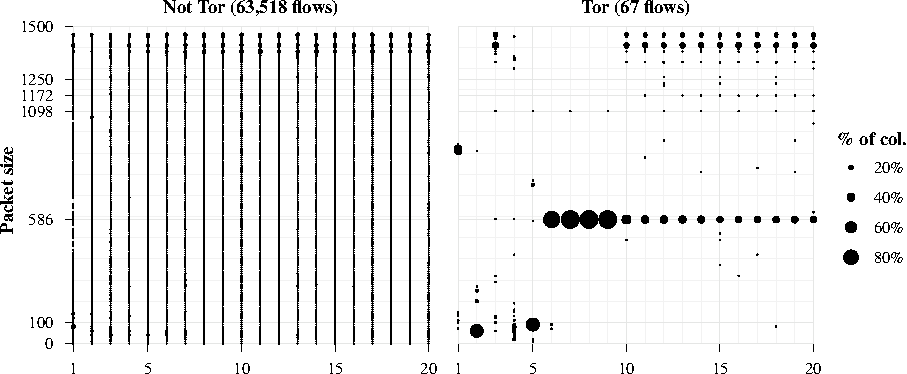
\includegraphics{figures/https-patterns-c}
\caption{Payload lengths for the first 20 non-empty packets of 63,585
  unidirectional flows on TCP port 443, taken from the CAIDA
  2011-Chicago data set.~\cite{d-caida} Port 443 is officially assigned
  to HTTP over TLS, but Tor relays are sometimes configured to accept
  connections on this port. Scanning for 586-byte TCP payloads
  identifies 67~of the flows as probable Tor traffic.}\label{f:packetlengths}
\end{figure*}

\begin{figure*}[t!]
\centering
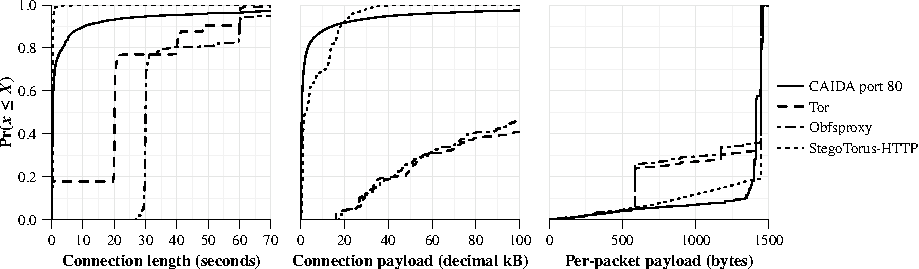
\includegraphics{plots/ecdf-cl-bw-pl}
\caption{Empirical CDFs of connection length, total data transferred,
  and per-packet payload for 20 visits to each of the Alexa top ten
  websites, using Tor directly (dashed line), obfsproxy (dot-dash
  line), and StegoTorus-HTTP (dotted line).  CAIDA Chicago-2011 port
  80 traffic for reference (solid line).} \label{fig:ECDFs}
\end{figure*}

\section{Detection Resistance}\label{s:attacks}

To evaluate how well StegoTorus can conceal a Tor stream, we developed
two attacks upon Tor, which StegoTorus ought to defeat if it is
functioning as intended.  We designed these attacks to be practical in
the resource-constrained environment of a perimeter filter (as
described in Section~\ref{s:limits-censor}) so they are deliberately
quite simple.  The first attack picks Tor streams out of other TCP
streams, based on a fundamental characteristic of the Tor wire
protocol that is cheap to detect.  The second attack operates on known
Tor streams and extracts information about the sites being visited
covertly.  In each case we will first describe the attack and how it
fares against Tor, then discuss its effectiveness against StegoTorus.
As we did for the steganography modules, we will also discuss
potential improvements to the attacks that might be implemented by an
adversary determined to detect StegoTorus.

\subsection{Detecting Tor}\label{s:detect-tor}

The Tor protocol~\cite{s-tor} sends nearly all messages in the form of
“cells” with a fixed length of 512 bytes.  These cells are packed into
TLS~1.0 application-data records~\cite{s-tls1} on the wire.  Because
of the “empty record” countermeasure for a cryptographic weakness in
TLS 1.0~\cite{a-ssl-cp1,a-ssl-cp2}, the overhead of TLS encapsulation
is 74 bytes per application-data record.  The client will pack many
cells into a record if it has enough to say, and TCP will split large
records in the middle in order to transmit MTU-sized packets, but Tor
nonetheless winds up transmitting many TCP packets that contain
exactly one cell.  These packets have a characteristic payload length
of 586 bytes.  A filtering router can pick Tor streams out of other
traffic by counting how often they appear.

We implemented the following concrete algorithm: let $\tau$ be the
adversary's current estimate of the probability that a given TCP flow
is Tor, initially set to zero.  Ignore packets containing only an ACK
and no payload; these are best treated as neutral~\cite{a-finger-onion}.
Otherwise, update
\(
\tau \leftarrow \alpha \tau + (1 - \alpha) \mathbf{1}_{l=586}
\)
where $\alpha \in (0,1)$ is a tuning parameter and
$\mathbf{1}_{l=586}$ is one if the TCP payload length $l$ equals 586
bytes, zero otherwise.  If $\tau$ rises past a threshold value $T$,
the TCP flow is considered Tor traffic.

To do this, a perimeter filter must be capable of tracking TCP flows
in realtime, and maintaining one scalar value (the estimate $\tau$)
for each; to the best of our knowledge, this is within the
capabilities of modern DPI hardware.  Empirically, $\alpha = 0.1$ and
$T = 0.4$ identifies Tor within a few dozen packets.
Figure~\ref{f:packetlengths} shows probable Tor flows picked out of
all the port-443 traffic in the CAIDA 2011-Chicago
data set~\cite{d-caida} with this technique.  (This data set only
includes IP and TCP headers for each packet captured, so we are unable
to confirm that the selected flows are actually Tor, or how much of
the background traffic is in fact HTTPS.)

To confirm the effectiveness of this attack against vanilla Tor, we
collected traffic traces from visiting the top ten Alexa sites twenty
times over vanilla Tor, obfsproxy~\cite{n-iran-ob}, and StegoTorus
with the \textit{HTTP} steganography module.  In addition to non-zero
TCP payload sizes for each packet, we extracted the lifetime and total
data transferred (treating the two directions as independent) of each
TCP stream.  Figure~\ref{fig:ECDFs} presents a qualitative comparison
of these features in the form of empirical CDFs, with all TCP flows on
port 80 of the CAIDA 2011-Chicago data set (again, we cannot confirm
this, but port 80 traffic on the public Internet is almost surely
HTTP) for reference.  Tor's predilection for generating 586-byte
packets is clearly seen in the rightmost panel of
Figure~\ref{fig:ECDFs}, and the other panels show other
characteristics that would be easy for the adversary to detect, such
as a tendency for TCP connections to last exactly 20 or 30 seconds.
Obfsproxy does little to alter these features.

StegoTorus fares much better.  It is not perfect, but it generates
empirical CDFs for all three features that are closer to the CAIDA
port 80 reference than they are to either Tor or obfsproxy.  In
particular, it eliminates the 586-byte characteristic payload size.
Still, a determined adversary with more analytic power at its disposal
might be able to detect the remaining statistical differences between
StegoTorus-HTTP and “normal” HTTP traffic that Figure~\ref{fig:ECDFs}
reveals.  Improving our HTTP emulation will reduce these differences.
If necessary, we could also implement an explicit statistical model of
what HTTP traffic “should” be like.
